\documentclass{article}

\usepackage{arxiv}

\usepackage[utf8]{inputenc} % allow utf-8 input
\usepackage[T1]{fontenc}    % use 8-bit T1 fonts
\usepackage{lmodern}        % https://github.com/rstudio/rticles/issues/343
\usepackage{hyperref}       % hyperlinks
\usepackage{url}            % simple URL typesetting
\usepackage{booktabs}       % professional-quality tables
\usepackage{amsfonts}       % blackboard math symbols
\usepackage{nicefrac}       % compact symbols for 1/2, etc.
\usepackage{microtype}      % microtypography
\usepackage{graphicx}

\title{The effects of job matching on employment accessibility measures
in the assessment of core public transport infrastructre}

\author{
    J Rafael Verduzco-Torres
    \thanks{Corresponding author. Email:
\href{mailto:JoseRafael.Verduzco-Torres@glasgow.ac.uk}{\nolinkurl{JoseRafael.Verduzco-Torres@glasgow.ac.uk}}.}
   \\
    Urban Studies \\
    University of Glasgow \\
  Hillhead, Glasgow G12 8RZ, United Kingdom \\
  \texttt{\href{mailto:JoseRafael.Verduzco-Torres@glasgow.ac.uk}{\nolinkurl{JoseRafael.Verduzco-Torres@glasgow.ac.uk}}} \\
   \And
    David Philip McArthur
   \\
    Urban Studies \\
    University of Glasgow \\
  Hillhead, Glasgow G12 8RZ, United Kingdom \\
  \texttt{\href{mailto:David.McArthur@glasgow.ac.uk}{\nolinkurl{David.McArthur@glasgow.ac.uk}}} \\
  }


% tightlist command for lists without linebreak
\providecommand{\tightlist}{%
  \setlength{\itemsep}{0pt}\setlength{\parskip}{0pt}}


% Pandoc citation processing
%From Pandoc 3.1.8
% definitions for citeproc citations
\NewDocumentCommand\citeproctext{}{}
\NewDocumentCommand\citeproc{mm}{%
  \begingroup\def\citeproctext{#2}\cite{#1}\endgroup}
\makeatletter
 % allow citations to break across lines
 \let\@cite@ofmt\@firstofone
 % avoid brackets around text for \cite:
 \def\@biblabel#1{}
 \def\@cite#1#2{{#1\if@tempswa , #2\fi}}
\makeatother
\newlength{\cslhangindent}
\setlength{\cslhangindent}{1.5em}
\newlength{\csllabelwidth}
\setlength{\csllabelwidth}{3em}
\newenvironment{CSLReferences}[2] % #1 hanging-indent, #2 entry-spacing
 {\begin{list}{}{%
  \setlength{\itemindent}{0pt}
  \setlength{\leftmargin}{0pt}
  \setlength{\parsep}{0pt}
  % turn on hanging indent if param 1 is 1
  \ifodd #1
   \setlength{\leftmargin}{\cslhangindent}
   \setlength{\itemindent}{-1\cslhangindent}
  \fi
  % set entry spacing
  \setlength{\itemsep}{#2\baselineskip}}}
 {\end{list}}
\usepackage{calc}
\newcommand{\CSLBlock}[1]{#1\hfill\break}
\newcommand{\CSLLeftMargin}[1]{\parbox[t]{\csllabelwidth}{#1}}
\newcommand{\CSLRightInline}[1]{\parbox[t]{\linewidth - \csllabelwidth}{#1}\break}
\newcommand{\CSLIndent}[1]{\hspace{\cslhangindent}#1}

\usepackage{float}
\usepackage{placeins}
\usepackage{amsmath}
\usepackage{setspace}
\doublespacing
\usepackage{graphicx} %Loading the package
\graphicspath{{../output/plot/}} %Setting the graphicspath
\usepackage{lscape}
\usepackage{booktabs}
\usepackage{longtable}
\usepackage{array}
\usepackage{multirow}
\usepackage{wrapfig}
\usepackage{float}
\usepackage{colortbl}
\usepackage{pdflscape}
\usepackage{tabu}
\usepackage{threeparttable}
\usepackage{threeparttablex}
\usepackage[normalem]{ulem}
\usepackage{makecell}
\usepackage{xcolor}
\begin{document}
\maketitle


\begin{abstract}
The definition of accessibility emphasizes the attractiveness of
opportunities that residents deem valuable. This study revises the
common assuption in empirical studies that residents are equally
attracted by all type of employment and its implication for public
transport evaluation. Additionally, the role of the modifiable problem
unit is also examined in this relationship.
\end{abstract}

\keywords{
    Employment accessibility
   \and
    Job matching
   \and
    Public transport infrastructure
   \and
    Modifiable areal unit problem
  }

\section{Introduction}\label{introduction}

Location-based accessibility measures are key to account for the level
of service offered by the transport infrastructure in a variety of
studies, including the property market or equity outcomes of large
public transport infrastructure projects. An elemental definition of
accessibility emphasizes the attractiveness of opportunities that
residents deem valuable. This study revises the common assumption in
empirical studies that residents are equally attracted by all type of
employment. Additionally, the role of the modifiable problem unit is
also examined in this relationship. These considerations can offer
useful guidance for the environmental measure of accessibility and its
application in environmental studies and the distribution of the
benefits of public transport infrastructure.

\begin{enumerate}
\def\labelenumi{\arabic{enumi}.}
\tightlist
\item
  What are the key spatial differences between generic and matching
  accessibility measures and what is the role of the MAUP?
\item
  How does the evaluation of PT infrastructure differs when accounting
  for matching employment opportunities in accessibility measures?
\item
  How do benefits of PT extensions differ between deprived or
  low-skilled populations and the general population when considering
  employment matching opportunities in accessibility?
\end{enumerate}

This paper contributes to literature by:

\begin{itemize}
\tightlist
\item
  Examining the spatial distribution of pubic transport benefits using
  accessibility measures by relaxing the assumption that all employment
  opportunities are equally attractive to all the population drawing on
  an empirical case in a ten-year period.
\item
  Examines the role of the MAUP in this effects.
\item
  Reports the findings of GMC, an understudied mega-city, by identifying
  and digitally reconstructing in a common format (general transit feed
  specification, GTFS) a series of temporal stages of the MPTN in GMC
  for a ten-year period (2009-2019).
\end{itemize}

\section{Literature review}\label{literature-review}

Thériault, Voisin, and Des Rosiers (2013) conceptualize accessibility as
``the ability that persons living in that area can, within an acceptable
travel time, reach a satisfactory diversity of activity locations that
are important to them'' (p.~234). Levinson and Wu (2020) simply put it
as ``the ease of reaching valued destinations'' (p.~130).

\subsection{Accessibility measures}\label{accessibility-measures}

formulation in Eq. \ref{eq:location-based1} incorporates: (1)
individual's profiles; 2) how different profiles perceive or experience
the space; and 3) constraints that may prevent segments of the
population to access some type of activities. Some of these individual
aspects involved in the construction of accessibility measures have been
found to be relevant in empirical studies. For instance, gender in
Osland (2010) or age and gender in Thériault, Voisin, and Des Rosiers
(2013) in the study of the property prices.

Equation \ref{eq:access-general} shows the formulation potential
accessibility to employment from location \(A_i\), which the
frequently-used in literature.

\begin{equation}
  A_{i} = \sum^N_{i=1} E_j f(c_{ij})
  \label{eq:access-general}
\end{equation}

The attractiveness of a destination is given by the number of employment
opportunities at \(j\), \(E_j\). \(f(c_{ij})\) is the impedance
affecting attractiveness as a function of travel cost between \(i\) and
\(j\). Frequently, travel cost is represented by the modelled travel
time.

In Eq. \ref{eq:eq:access-general}, households and opportunities are
assumed to be homogeneous, i.e., all types of employment are equally
attractive for all types of residents. Following contributions from
theory (Geurs and van Wee 2004; Levinson and Wu 2020), an extended
accessibility measure should take into consideration the characteristics
of the demand (residents at origins) and supply at potential
destinations. In the context of the labour market, this idea is
supported by the Human Capital Theory (Schultz 1961; Becker 1994).

There are different versions of its operationalization in existing
empirical studies (e.g. Pereira, Grégoire, and Karner 2019). For
instance, these characteristics can be expressed as type of person \(m\)
at \(j\) and type of employment \(m\) at \(k\). Accordingly, the measure
can be specified as following:

\begin{equation}
  A_{im} = \sum^N_{i=1} E_{im} f(c_{ij}),
   \label{eq:access-matching}
\end{equation}

Here, only employment opportunities \(E\) matching the profile of
residents between \(j\) and \(k\) are considered. Thus, this reflect the
notion that residents would find attractive only employment
opportunities that match their skills and education level with a
relevant employment opportunity.

\subsubsection{Evaluation of public
transport}\label{evaluation-of-public-transport}

Location-based accessibility measures have been used to evaluate the
performance of public transport systems in policy report and research
(Ermagun 2021; Liu, Porr, and Miller 2022; Conway, Byrd, and Van
Eggermond 2018; Malekzadeh and Chung 2020; Palmateer et al. 2021). A
measure based on realistic travel times can reflect important elements
of a public transport system. This is because travel time by public
transport is affected by several aspects of the system, such as:

\begin{itemize}
\tightlist
\item
  The topology of the network, e.g.~connectivity, centrality.
\item
  Capacity of the infrastructure, e.g.~degree of right of way
  segregation, capacity and design of stations.
\item
  Spatial coverage, e.g.~availability of infrastructure and catchment
  areas.
\item
  Operational characteristics, e.g.~frequency of services, overlapping
  routes, express services, transfer wait times.
\end{itemize}

Despite the growing relevance of accessibility measures in the
evaluation of public transport infrastructure, knowledge of the
implications of overlooking matching employment are limited in
literature.

\section{Methods}\label{methods}

\subsection{Accessibility measures
examined}\label{accessibility-measures-examined}

The general accessibility is computed as following for this work:

\begin{equation}
  A^{\text{PT}}_{jt} = \sum^J_{j=1} E_k f(d_{jkt})
   \label{eq:empirical-access-general}
\end{equation}

The implementation of matching accessibility is adapted according to the
information available for the area of study and some preliminary
findings. The households' education level (i.e., median number of years
of education) is employed assuming correspondence with the level of
salary paid in the employment market. This is further supported by the
positive relationship found between education level and wages in
empirical studies in the context of Mexico (Nuñez, Paredes, and
Garduño-Rivera 2017; Rojas, Angulo, and Velázquez 2000).

\begin{equation}
  A^{\text{PT}}_{jtm} = \sum^J_{j=1} E_{km} f(d_{jkt}),
   \label{eq:empirical-access-matching}
\end{equation}

Here, \(m\) at \(j\) is categorized according to the median education
level of its residents by quintile and \(m\) at \(k\) is classified
based on the average paid salary by quintile. Only employment
opportunities \(E\) matching the education level quantile between \(j\)
and \(k\) are considered (when \(j \ne k\)).\footnote{An exception
  occurs when \(j = k\). In this case, employment opportunities in the
  origin are considered as available. This is to avoid the assumption
  implying that some zones have accessibility values equal to 0} This
assumes that residents would deem valuable only employment opportunities
that match their education level, i.e.~those in the same quintile. The
data sources and specific procedures to process the data are described
in the next sub-section.

\subsection{Area of study}\label{area-of-study}

Greater Mexico City (GMC) (\emph{Zona Metropolitana del Valle de
México}) is located in in the south-centre of Mexico. In 2015, GMC had
nearly 21 million inhabitants (INEGI 2015b). The official delimitation
consists of 76 adjacent municipalities, which are part of three
different states, namely: (1) \emph{Ciudad de México} (16
municipalities); (2) \emph{Hidalgo} (1 municipality), and (3)
\emph{México} (59 municipalities). The total GMC area is 7,889
km\textsuperscript{2}, and it is home to 17\% of the national
population.

\subsubsection{The main public transport network
(MPTN)}\label{the-main-public-transport-network-mptn}

The focus of this work is on \emph{rapid transit} and \emph{semi-rapid
transit} infrastructure, excluding specialized modes i.e.~\emph{aerial
tramway}. The combination of public transport modes included in the
analyses is referred to as the \emph{main public transport network}
(MPTN). Figure \ref{fig:metro-map} shows the MPTN in GMC for the year
2019. This consists of a variety of modes operated by the following main
agencies: The metro system, directly operated by the state-owned company
\emph{Sistema de Transporte Colectivo} (STC) and designated as Metro;
two BRT systems, namely \emph{Metrobus} (MB) in Ciudad de México and
Mexibus (MXB) in the state of México; One LRT line operated by STE; and
one regional rail line designated as \emph{Sub}.

\begin{figure}
  \centering
  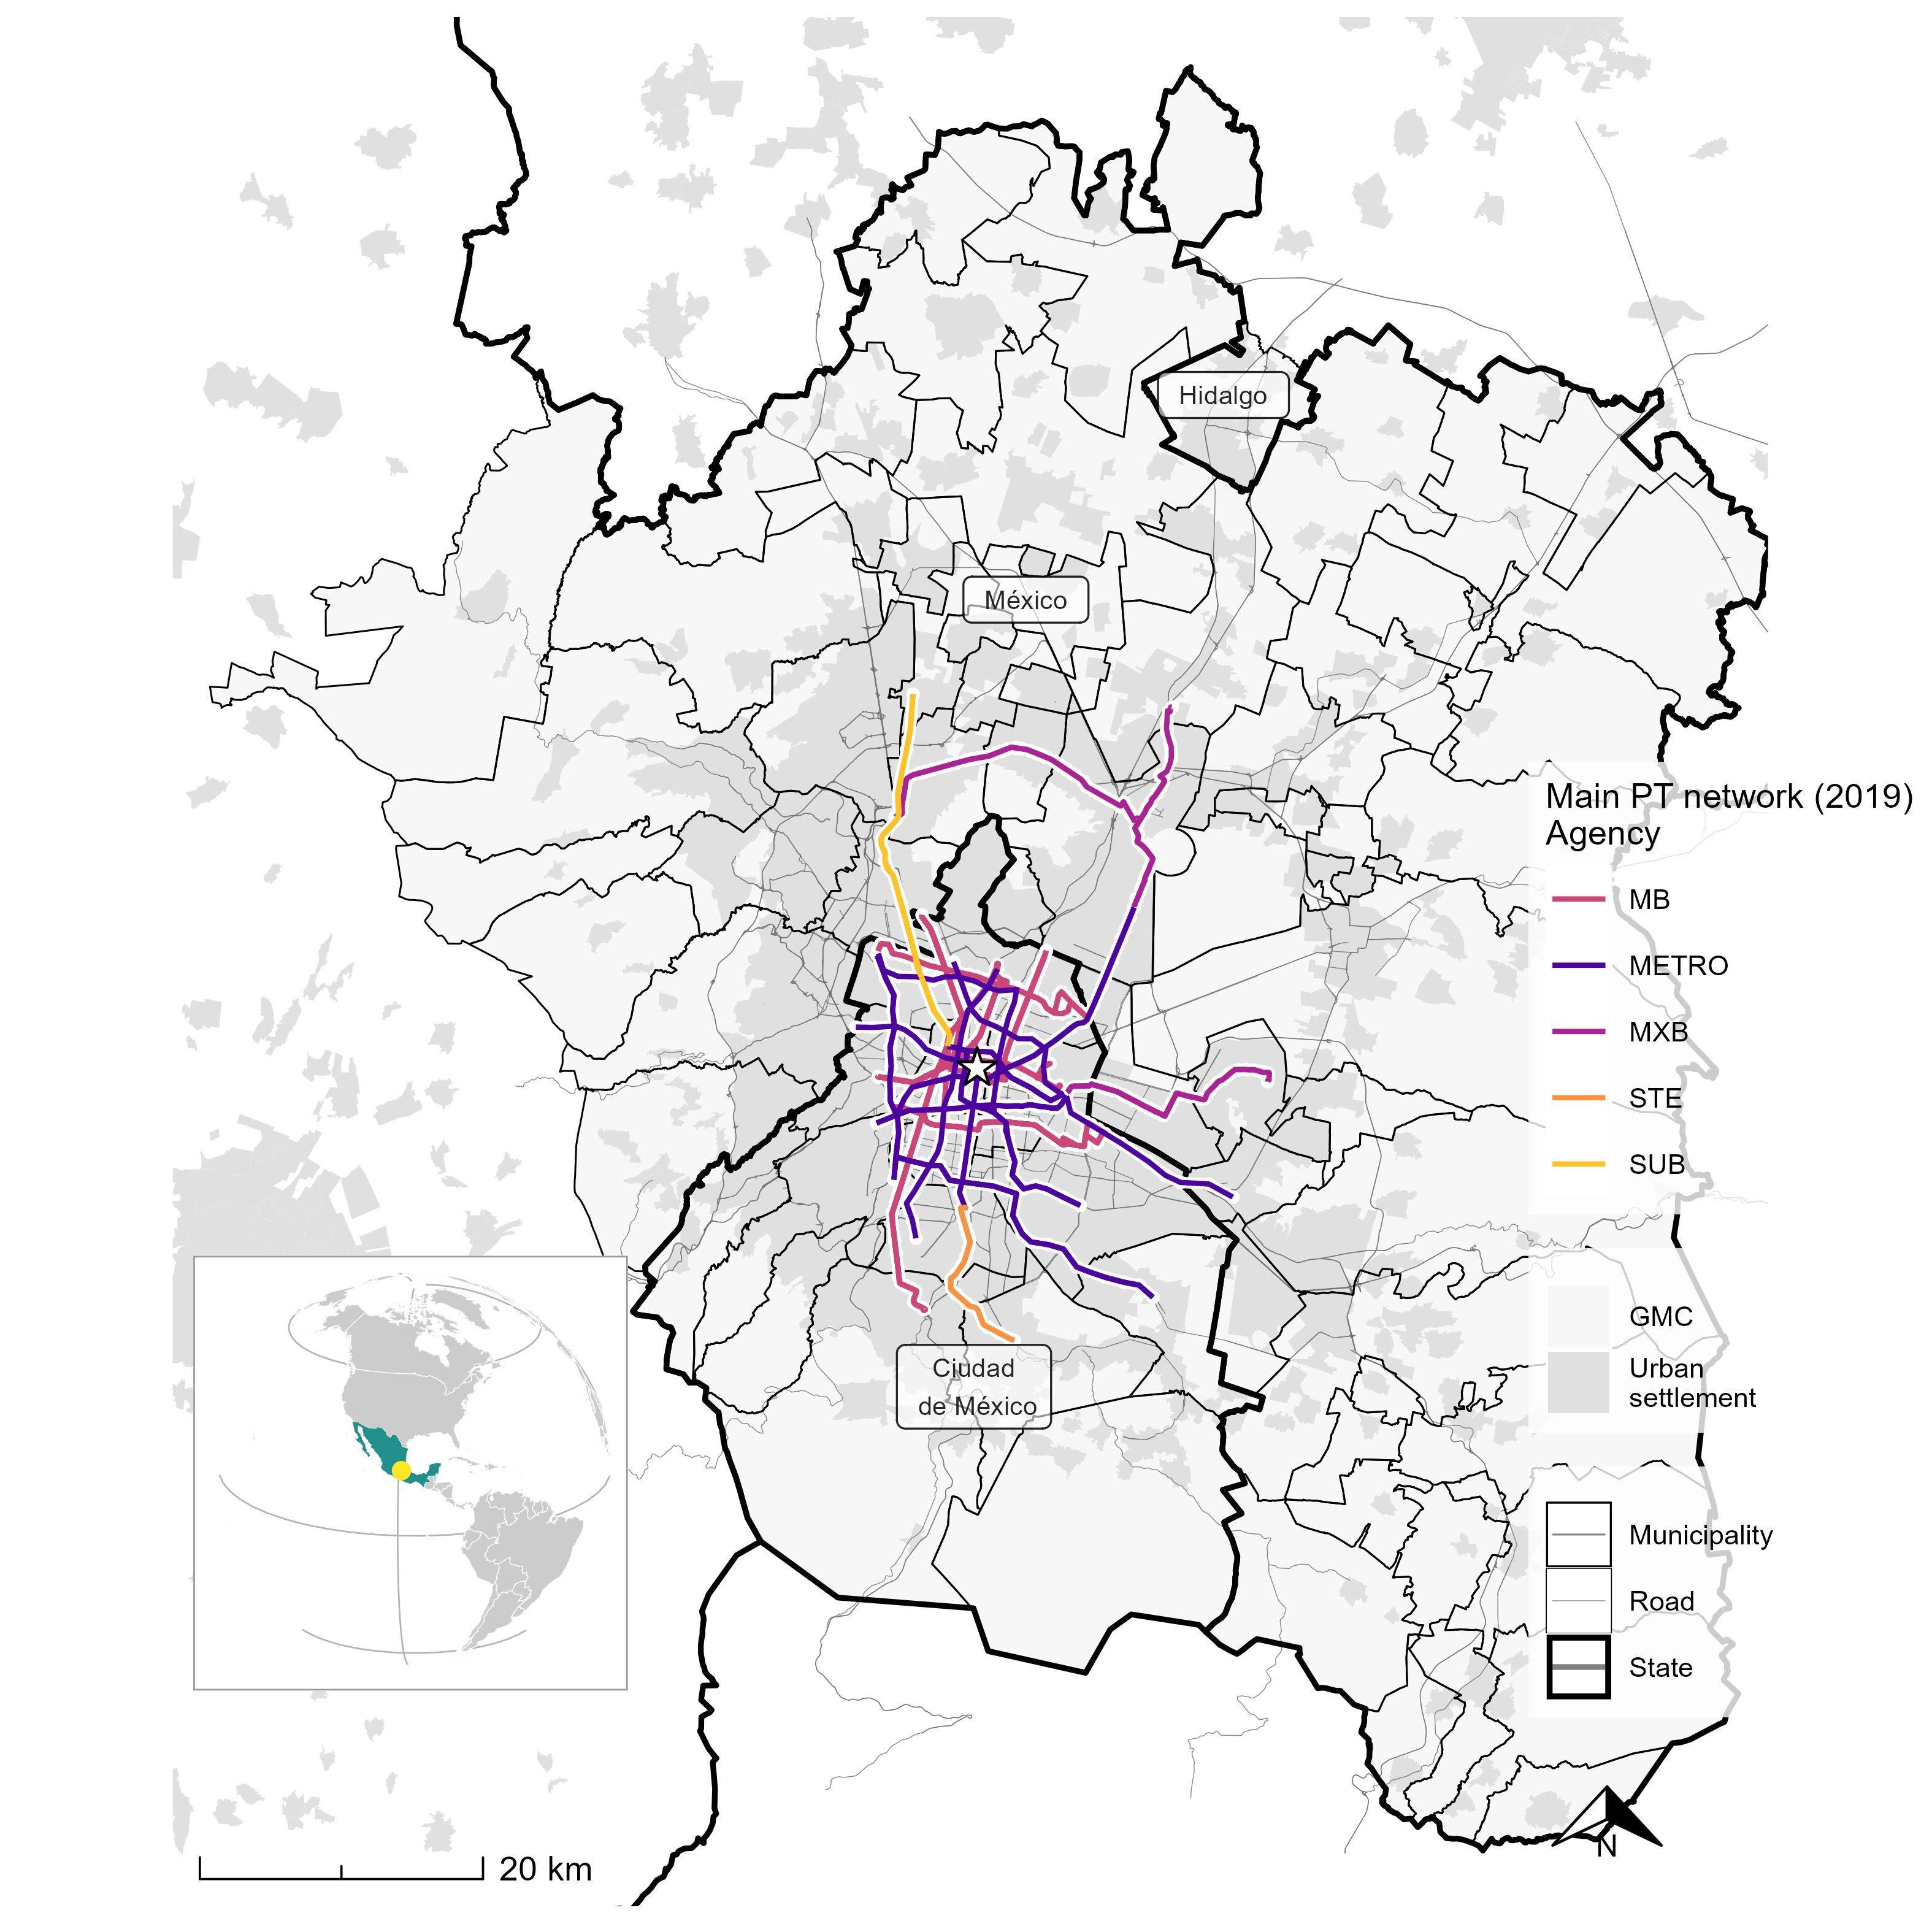
\includegraphics[width=0.9\textwidth]{figures/metro_map.png}
  \caption{Main public transport network (MPTN). Greater Mexico City, 2019.}
  \footnotesize{\textit{Source:} Verduzco-Torres (2023) based on Marco Geoestadístico Nacional 2014 Versión 6.2 (INEGI, 2014); Delimitación de las zonas metropolitanas México 2015 (INEGI, 2018); Secretaría de Movlidad de la Ciudad de México (SEMOVI, n.d.); Sistema de Transporte Masivo y Teleférico del Estado de México (SITRAMyTEM, n.d.); OpenStreetMap (OSM, n.d.).}
  \label{fig:metro-map}
\end{figure}

The period of study was divided into seven temporal stages to reflect
significant changes in the MPTN over time. Initially, changes were
identified by the physical alterations in the MPTN, such as the opening
of a new corridor or the extension of an existing one. Table
\ref{tab:stages-network} details these changes and their corresponding
temporal stages from 2010 to 2019. The stages were grouped based on the
time interval between changes, with modifications occurring within six
months being grouped together in the same stage. This criteria follows
previous empirical studies and assumes that accessibility benefits are
perceived as simultaneous when changes happen within short timeframes
(Ahlfeldt 2013; Gibbons and Machin 2005).

\begin{table}
\centering
\caption{\label{tab:stages-network}Main public transport network extensions between 2010 and 2019 in Greater Mexico City grouped by temporal stage.}
\centering
\fontsize{9}{11}\selectfont
\begin{tabular}[t]{ll>{\raggedright\arraybackslash}p{8em}>{\raggedright\arraybackslash}p{8em}>{\raggedright\arraybackslash}p{8em}>{\raggedright\arraybackslash}p{4em}l}
\toprule
Corridor & Agency & From station & To station & Opening date & Previous change* & GTFS source\\
\midrule
\addlinespace[0.3em]
\multicolumn{7}{l}{\textit{\textbf{Stage 7: 2018 to 2019}}}\\
\hspace{1em}7 & MB & Indio Verdes & Campo Marte & 2018-03-01 & 26 & 2019-01-09\\
\addlinespace[0.3em]
\multicolumn{7}{l}{\textit{\textbf{Stage 6: 2016 to 2018}}}\\
\hspace{1em}6 & MB & El Rosario & Martín Carrera & 2016-01-01 & 12 & 2017-09-02\\
\addlinespace[0.3em]
\multicolumn{7}{l}{\textit{\textbf{Stage 5: 2015 to 2016}}}\\
\hspace{1em}2 & MXB & La Quebrada & Las Americas & 2015-01-01 & 14 & 2015-01-28\\
\addlinespace[0.3em]
\multicolumn{7}{l}{\textit{\textbf{Stage 4: 2013 to 2015}}}\\
\hspace{1em}5 & MB & Río de los Remedios & San Lázaro & 2013-11-01 & 6 & 2014-12-30\\
\hspace{1em}3 & MXB & Chimalhuacán & Pantitlán & 2013-05-01 & 7 & 2014-12-30\\
\addlinespace[0.3em]
\multicolumn{7}{l}{\textit{\textbf{Stage 3: 2012 to 2013}}}\\
\hspace{1em}12 & Metro & Mixcoac & Tlahuac & 2012-10-01 & 6 & 2013-10-21\\
\hspace{1em}4 & MB & Buenavista & San Lazaro Aeropuerto & 2012-04-01 & 14 & 2013-10-21\\
\addlinespace[0.3em]
\multicolumn{7}{l}{\textit{\textbf{Stage 2: 2010 to 2012}}}\\
\hspace{1em}3 & MB & Tenacayuca & Etiopia & 2011-02-01 & 4 & 2013-10-21\\
\hspace{1em}1 & MXB & Ciudad Azteca & Ojo de Agua & 2010-10-01 & 10 & 2013-10-21\\
\addlinespace[0.3em]
\multicolumn{7}{l}{\textit{\textbf{Stage 1: Before 2010}}}\\
\hspace{1em}2 & MB & Tepalcates & Tacubaya & 2009-12-01 & NA & 2013-10-21\\
\bottomrule
\multicolumn{7}{l}{\rule{0pt}{1em}\textit{Note: }}\\
\multicolumn{7}{l}{\rule{0pt}{1em}*Months relative to the previous modification of the main public transport network.}\\
\end{tabular}
\end{table}

The MPTN stages and corresponding corresponding corridors are in Figure
\ref{fig:evolution-network}.

\begin{figure}
  \centering
  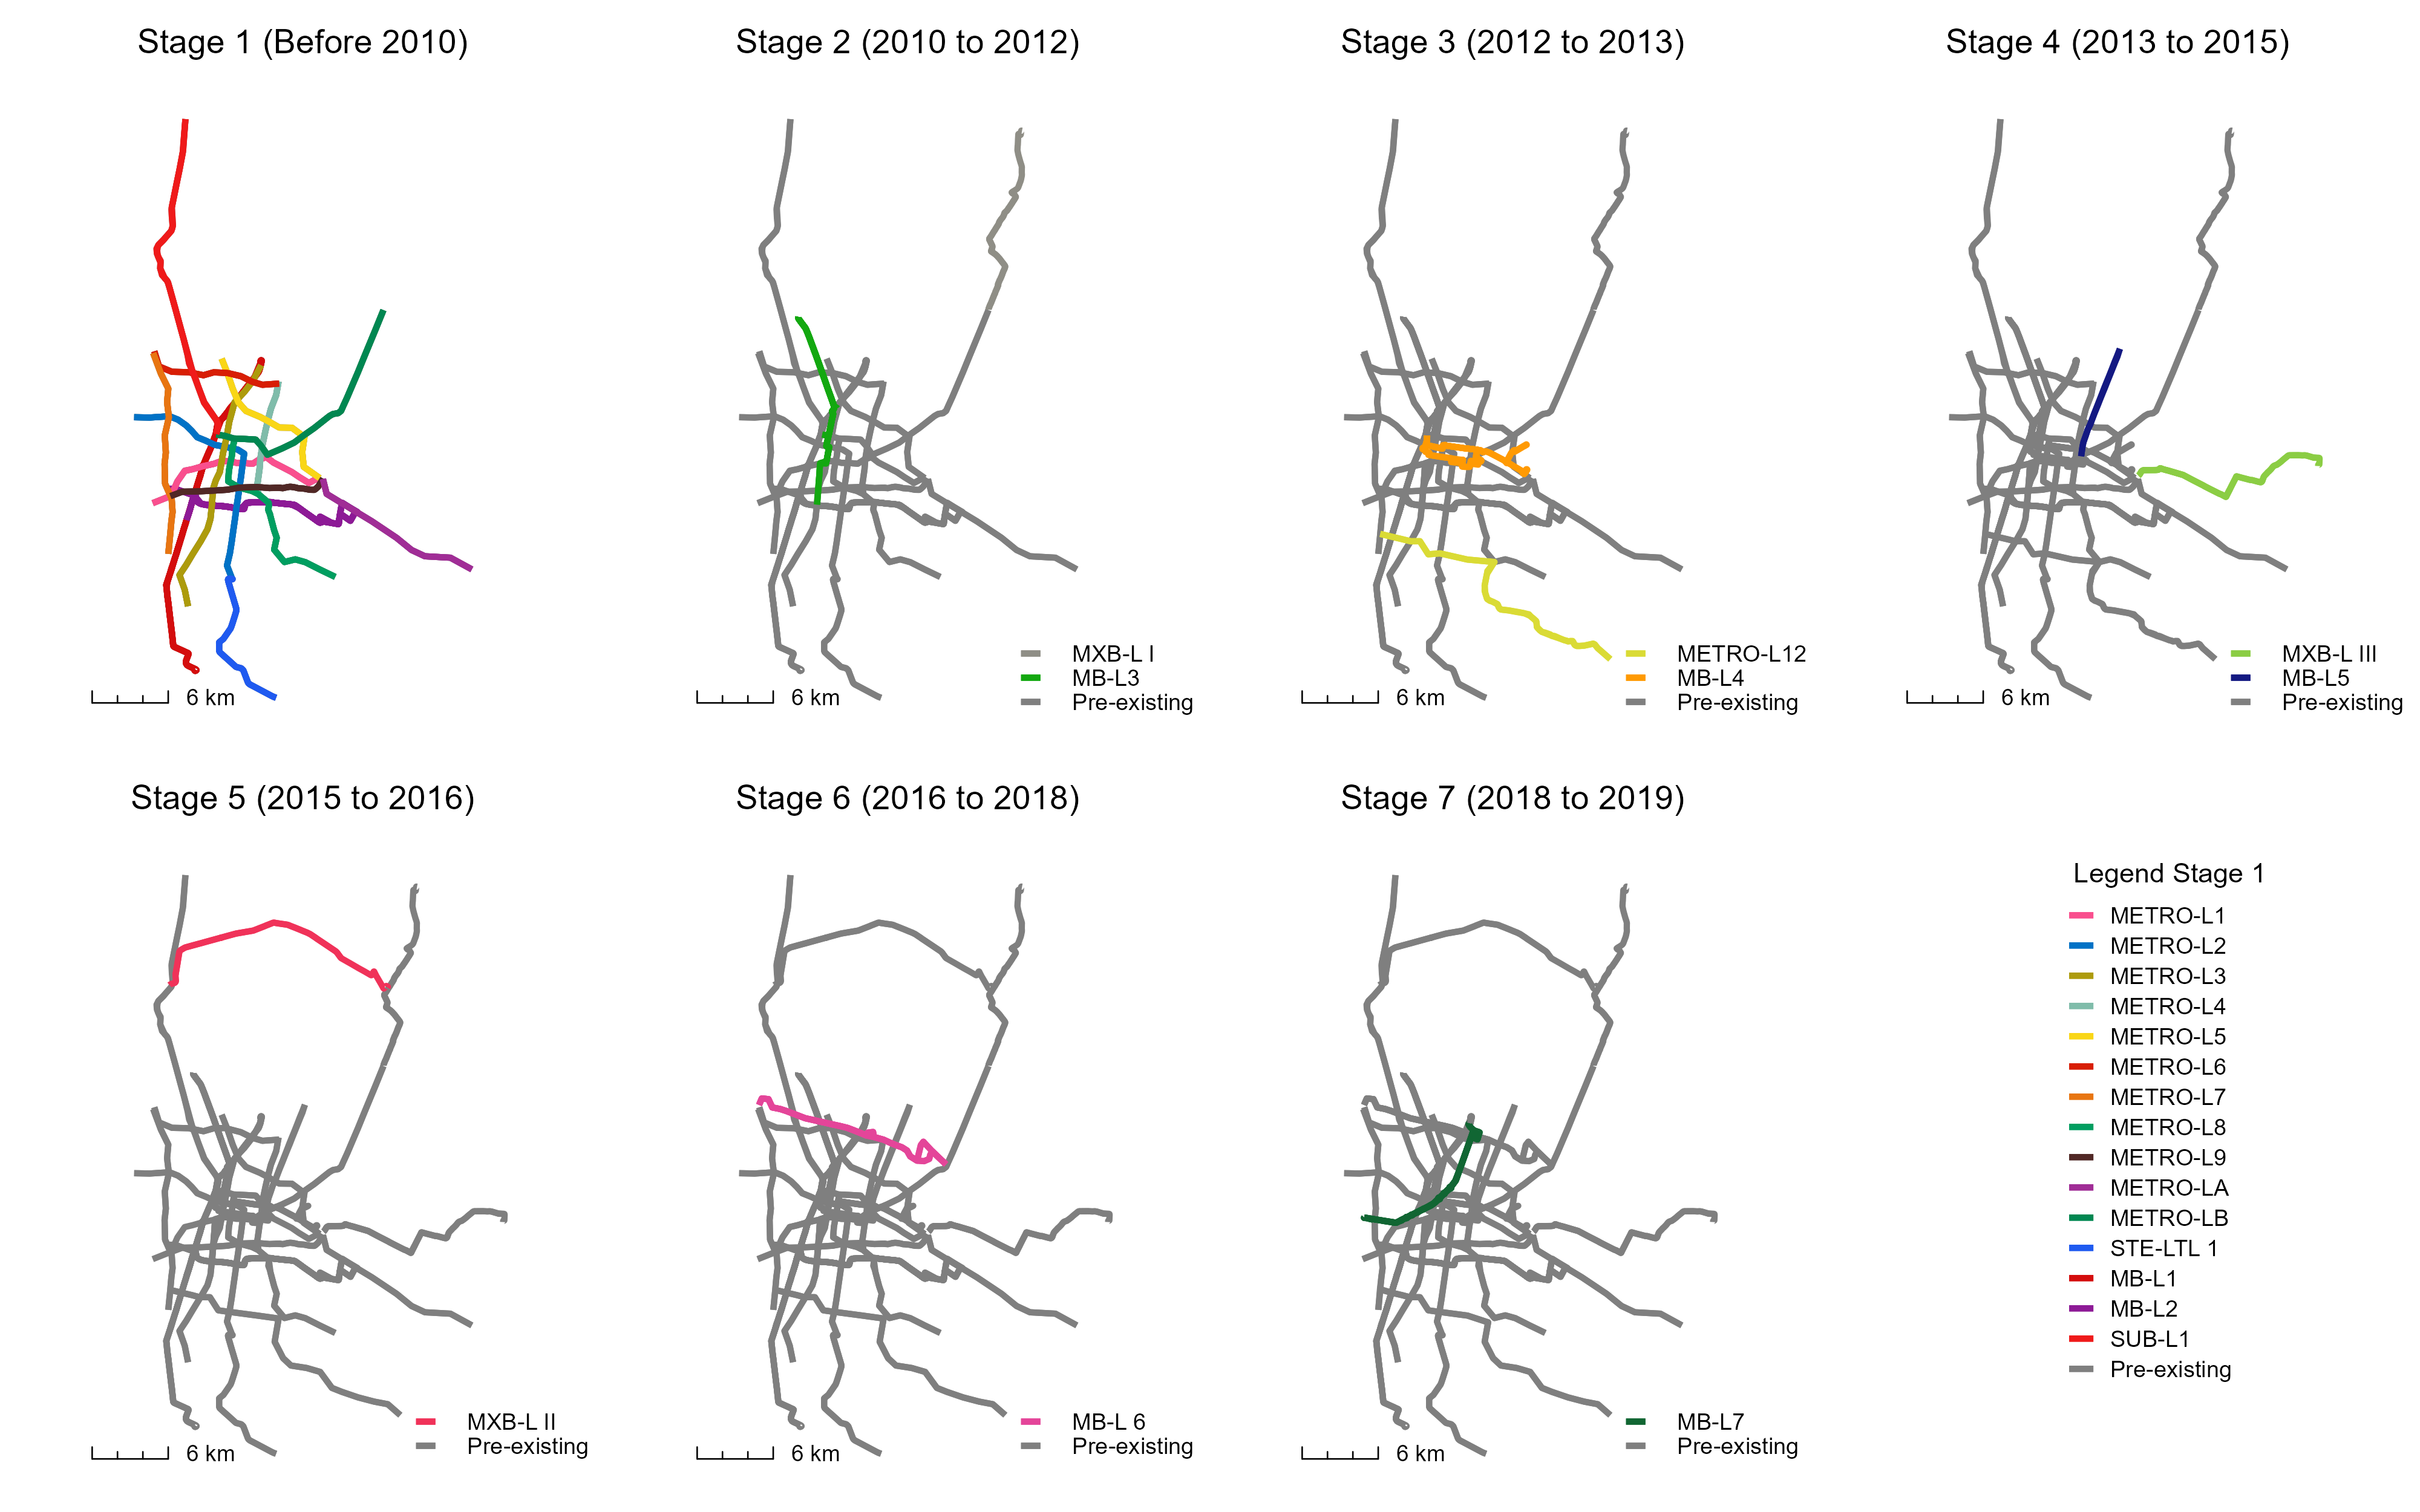
\includegraphics[width=0.95\textwidth]{figures/evo_transit_network.png}
  \caption{Temporal stages of the main public transport network. Greater Mexico City, 2010 to 2019.}
  \footnotesize{\textit{Source:} The author based on Semovi (n.d.) and SITRAMyTEM (n.d.).}
  \label{fig:evolution-network}
\end{figure}

\subsection{Data}\label{data}

\subsubsection{Demographics}\label{demographics}

The demographic data employed to account for person components in
accessibility measures come from the 2010 Population Census (INEGI
2012). These data were selected for their detailed disaggregation at the
city block level, including key fields such as total population and
average years of education completed by individuals aged 15 and older.

The count data included were transferred to the SAS using the
\emph{areal weighting method} (Saporito et al. 2007). This reassigns the
data according to the proportional overlay of the source and target
areas. The average education level was assigned using the
\emph{population weighting method}. In addition, this takes into
consideration the number of inhabitants and their type.

\subsubsection{Employment}\label{employment}

Employment data are sourced from the 2014 Economic Census (\emph{Censos
Económicos 2014}) (INEGI 2015b) and accessed at the city block level via
the Microdata Lab and Remote Processing service
(\url{https://www.inegi.org.mx/microdatos/}). The dataset includes: 1.
Number of establishments (fixed locations producing goods or services);
2. Employed personnel (individuals active in establishments, including
volunteers and family members), referred to as `employment'; and 3.
Total gross remuneration paid for the relevant year.

Employment information which came aggregated at higher geographic level
than the city-block due to privacy (\textless8\%) were re-allocated
using proportional estimates based on the spatial distribution from the
2015 DENUE (INEGI 2015a). This is an open-access, point-level dataset of
individual establishments. The employment data was assigned from city
blocks to SASs following the same approach employed for the demographic
data, i.e.~according to the areal weighting method.

The average income was computed for each areal unit based on the total
number of employment and the total gross remuneration paid.

\subsubsection{Public transport
itineraries}\label{public-transport-itineraries}

The estimated travel time used for accessibility measures is based on
scheduled public transport services. The Transport Authority in Mexico
City (\emph{Secretaría de Movilidad de la Ciudad de México}, Semovi)
released the first \emph{general transit feed specification} (GTFS)
files in 2013, which were accessed via the Open Mobility website
(\url{https://openmobilitydata.org/}). These datasets cover the agencies
operating most MPTN services in GMC. However, there are some
limitations: firstly, the geographic coverage primarily includes
services within Ciudad de México, excluding BRT services provided by
MXB. Secondly, the temporal coverage starts in 2013, with updates
occurring only sporadically, approximately once a year.

To overcome the first limitation, the geographic coverage of the
official GTFS data was augmented to include three BRT corridors operated
by MXB. This was carried out \emph{manually} based on unstructured
information provided by the Transport Agency of the State of Mexico
(\emph{Sistema de Transporte Masivo y Teleferico del Estado de México},
Sitramytem). This corresponded to services for 2019 only.

Regarding the second limitation, the MPTN's temporal stages were
reconstructed using the GTFS standard. The primary input for each stage
was the closest available official GTFS data reflecting changes in the
MPTN, with only the relevant services for each corridor in their
respective stages being retained. For MXB services, 2019 data was
considered due to the lack of earlier details, assuming uniform
characteristics of the BRT corridors across the stages. Similarly, for
other corridors included in early stages, services were assumed to
reflect 2013 levels due to the unavailability of earlier data. All
non-MPTN services were excluded, thereby focusing exclusively on the
benefits of the MPTN.

\subsubsection{Road network and pedestrian
infrastructure}\label{road-network-and-pedestrian-infrastructure}

The road and pedestrian infrastructure network is sourced from
\emph{OpenStreetMap} (OSM) (Manually downloaded on 30th October 2019
through a web export tool available in
\url{https://export.hotosm.org/es/v3/}{]}). This enables multi-modal
journeys to realistically represent the access/egress stage to a public
transport service when combining walking and public transport.

\subsection{Travel costs and impedance
parameters}\label{travel-costs-and-impedance-parameters}

\subsubsection{Modeled travel time}\label{modeled-travel-time}

Travel time matrices were calculated for each origin-destination (OD)
pair across SASs using a combination of walking and public transport
within the main public transport network. OD points \(i\) and \(j\) are
represented by population-weighted centroids of spatial units containing
economic activity (from the 2014 Economic Census) or demographic data
(from the 2010 Population Census). Travel times are capped at 180
minutes, based on patterns observed in the 2017 Travel Survey.

Travel times were modelled using a door-to-door approach with
OpenTripPlanner (OTP) version `1.4.0' (OTP n.d.) via the implementation
of an open-access routine written \texttt{Python} (Pereira et al. 2019).
This approach considers access, waiting, onboard, transfer, and egress
times. All-to-all travel time matrices were generated for each SAS
across seven temporal stages using reconstructed GTFS files and
road/pedestrian networks, with eight random departure times between 10
a.m. and 2 p.m. The median travel time was used for accessibility models
(Conway, Byrd, and van der Linden 2017). This process, computationally
intensive due to the high resolution of SASs, resulted in 2.1 billion
routes. Matrices were then merged, and median travel times calculated,
with walking distances limited to 3 km when using public transport and
4.8 km (60 minutes) for walking-only trips.

The internal-zone travel-times were estimated based on the surface area
as following: \(d_{i=j} = \frac{1}{2} \sqrt{ \frac{area_i}{\pi}}\)
(Frost and Spence 1995; Stepniak and Rosik 2015). The metric distance
was transformed to travel time using the average speed modelled for
short journeys (less than 3 km).

\subsubsection{Spatial Decaying Function and Calibration of
Accessibility
Parameters}\label{spatial-decaying-function-and-calibration-of-accessibility-parameters}

The spatial decaying function and parameters for accessibility measures
were determined using estimates from a trip distribution model,
following Handy and Niemeier (1997). This model is used to understand
how commuters in Greater Mexico City (GMC) discount employment
opportunities based on travel time. The analyses use data from the 2017
Travel Survey, focusing on weekday public transport and walking trips.

A series of alternative specifications were estimated within a doubly
constrained gravity model framework, expressed as following:

\begin{equation}
  T_{jk} = A_j O_j B_k D_k f(d_{jk})
  \label{eq:gravity-model}
\end{equation}

where \begin{equation} 
  A_j = \left[ \sum{B_i D_i f(d_{jk})} \right]^{-1}
\end{equation}

and \begin{equation} 
  B_k = \left[ \sum{A_k O_k f(d_{jk}) }  \right] ^{-1}
\end{equation}

with balancing factors \(A_j\) and \(B_k\) calculated iteratively. The
model estimates commuter flows (\(T_{jk}\)) between origins (\(j\)) and
destinations (\(k\)), with constraints on the number of journeys at
each. \(f(d_{jk})\) is a spatial deterrence or decaying function. The
inverse power (\(d_{jk}^{-\beta}\)) and negative exponential
(\(e^{(-\beta d_{jk})}\)) decaying functions were tested. \(\beta\)
represents the deterrence parameter.

A modified specification intended to capture an add-up cost for
inter-zone journeys or analogously a benefit of residing and working
within the same zone is considered (Thorsen and Gitlesen 1998). This
includes a parameter \(\mu\) which affects only the diagonal elements of
the OD matrix. The term is given by the following expression:

\begin{equation} 
  \mu \delta_{jk}
\end{equation}

where Kronecker delta takes the following value:

\begin{equation}
  \delta_{ij} \left\{
    \begin{array}{ll}
        0 & \quad \text{if   } j \neq k \\
        1 & \quad \text{if   } j = k \\
    \end{array} 
   \right.\\
\end{equation}

The simultaneous calibration of the model parameters \(\beta\) and
\(\mu\) is achieved via optimization by minimizing the standardized root
mean square error (SRMSE) using the \emph{Nelder-Mead's simplex
algorithm} as implemented in base \texttt{R} (\textbf{R-base?}).

The preliminary analyses shows that the negative exponential function
provided more accurate estimates compared to the inverse power. Also,
the use of the within-zone parameter \(\mu\) improves the estimates.
Therefore, the selected specification is the modified negative
exponential including \(\mu\). The parameters employed to estimate
accessibility are shown in Table \label{tab:access-pars}.

\section{Results}\label{results}

\FloatBarrier

\section{Conclusions}\label{conclusions}

\FloatBarrier

\section*{References}\label{references}
\addcontentsline{toc}{section}{References}

\phantomsection\label{refs}
\begin{CSLReferences}{1}{0}
\bibitem[\citeproctext]{ref-Ahlfeldt2013}
Ahlfeldt, Gabriel M. 2013. {``If We Build It, Will They Pay? Predicting
Property Price Effects of Transport Innovations.''} \emph{Environment
and Planning A} 45 (8, 8): 1977--94.
\url{https://doi.org/10.1068/a4549}.

\bibitem[\citeproctext]{ref-Becker1994}
Becker, Gary S. 1994. \emph{Human {Capital}: {A Theoretical} and
{Empirical Analysis} with {Special Reference} to {Education}}. 3rd ed.
Chicago: The University of Chicago Press.

\bibitem[\citeproctext]{ref-Conway2017}
Conway, Matthew Wigginton, Andrew Byrd, and Marco van der Linden. 2017.
{``Evidence-{Based Transit} and {Land Use Sketch Planning Using
Interactive Accessibility Methods} on {Combined Schedule} and
{Headway-Based Networks}.''} \emph{Transportation Research Record:
Journal of the Transportation Research Board} 2653 (1, 1): 45--53.
\url{https://doi.org/10.3141/2653-06}.

\bibitem[\citeproctext]{ref-Conway2018}
Conway, Matthew Wigginton, Andrew Byrd, and Michael Van Eggermond. 2018.
{``Accounting for Uncertainty and Variation in Accessibility Metrics for
Public Transport Sketch Planning.''} \emph{Journal of Transport and Land
Use} 11 (1, 1). \url{https://doi.org/10.5198/jtlu.2018.1074}.

\bibitem[\citeproctext]{ref-Ermagun2021}
Ermagun, Alireza. 2021. {``Transit Access and Urban Space-Time Structure
of {American} Cities.''} \emph{Journal of Transport Geography} 93 (May).
\url{https://doi.org/10.1016/j.jtrangeo.2021.103066}.

\bibitem[\citeproctext]{ref-Frost1995}
Frost, M. E., and N. A. Spence. 1995. {``The Rediscovery of
Accessibility and Economic Potential: The Critical Issue of
Self-Potential.''} \emph{Environment \& Planning A} 27 (11, 11):
1833--48. \url{https://doi.org/10.1068/a271833}.

\bibitem[\citeproctext]{ref-Geurs2004}
Geurs, Karst T., and Bert van Wee. 2004. {``Accessibility Evaluation of
Land-Use and Transport Strategies: {Review} and Research Directions.''}
\emph{Journal of Transport Geography} 12 (2, 2): 127--40.
\url{https://doi.org/10.1016/j.jtrangeo.2003.10.005}.

\bibitem[\citeproctext]{ref-Gibbons2005}
Gibbons, Stephen, and Stephen Machin. 2005. {``Valuing Rail Access Using
Transport Innovations.''} \emph{Journal of Urban Economics} 57 (1, 1):
148--69. \url{https://doi.org/10.1016/j.jue.2004.10.002}.

\bibitem[\citeproctext]{ref-Handy1997}
Handy, Susan L, and Deb A Niemeier. 1997. {``Measuring Accessibility: An
Exploration of Issues and Alternatives.''} \emph{Environment and
Planning A} 29 (7, 7): 1175--94. \url{https://doi.org/10.1068/a291175}.

\bibitem[\citeproctext]{ref-INEGI2012}
INEGI. 2012. {``Sistema Para La {Consulta} de {Información Censal}
({SCINCE}).''} Instituto Nacional de Estadística y Geografía. 2012.
\url{https://www.inegi.org.mx/app/descarga/?ti=13&ag=01}.

\bibitem[\citeproctext]{ref-INEGI2015a}
---------. 2015a. {``Directorio {Estadístico Nacional} de {Unidades
Económicas} 2015.''} 2015. \url{https://www.inegi.org.mx/default.html}.

\bibitem[\citeproctext]{ref-INEGI2015}
---------. 2015b. {``Encuesta {Intercensal} 2015.''} 2015.
\url{https://www.inegi.org.mx/programas/intercensal/2015/}.

\bibitem[\citeproctext]{ref-Levinson2020}
Levinson, David M, and Hao Wu. 2020. {``Towards a General Theory of
Access.''} \emph{Journal of Transport and Land Use} 13 (1, 1): 129--58.
\url{https://doi.org/10.5198/jtlu.2020.1660}.

\bibitem[\citeproctext]{ref-Liu2022}
Liu, Luyu, Adam Porr, and Harvey J. Miller. 2022. {``Realizable
Accessibility: Evaluating the Reliability of Public Transit
Accessibility Using High-Resolution Real-Time Data.''} \emph{Journal of
Geographical Systems}, May.
\url{https://doi.org/10.1007/s10109-022-00382-w}.

\bibitem[\citeproctext]{ref-Malekzadeh2020}
Malekzadeh, Ali, and Edward Chung. 2020. {``A Review of Transit
Accessibility Models: {Challenges} in Developing Transit Accessibility
Models.''} \emph{International Journal of Sustainable Transportation} 14
(10, 10): 733--48. \url{https://doi.org/10.1080/15568318.2019.1625087}.

\bibitem[\citeproctext]{ref-Nunez2017}
Nuñez, Hector M., Dusan Paredes, and Rafael Garduño-Rivera. 2017. {``Is
Crime in {Mexico} a Disamenity? {Evidence} from a Hedonic Valuation
Approach.''} \emph{Annals of Regional Science} 59 (1, 1): 171--87.
\url{https://doi.org/10.1007/s00168-017-0823-8}.

\bibitem[\citeproctext]{ref-Osland2010a}
Osland, Liv. 2010. {``Spatial Variation in Job Accessibility and Gender:
{An} Intraregional Analysis Using Hedonic House-Price Estimation.''}
\emph{Environment and Planning A} 42 (9, 9): 2220--37.
\url{https://doi.org/10.1068/a42422}.

\bibitem[\citeproctext]{ref-OTP}
OTP. n.d. {``{OpenTripPlanner}.''} Accessed October 10, 2019.
\url{https://www.opentripplanner.org/}.

\bibitem[\citeproctext]{ref-Palmateer2021}
Palmateer, Chelsey, Andrew Owen, David M Levinson, and Alireza Ermagun.
2021. {``The {Role} of {Transit Service Area Definition} for
{Access-based Evaluation}.''} In \emph{Applications of {Access}}.
Sidney: The University of Sidney.

\bibitem[\citeproctext]{ref-Pereira2019a}
Pereira, Rafael H M, David Banister, Tim Schwanen, and Nate Wessel.
2019. {``Distributional Effects of Transport Policies on Inequalities in
Access to Opportunities in {Rio} de {Janeiro}.''} \emph{Journal of
Transport and Land Use} 12 (1 SE -, 1 SE -).
\url{https://doi.org/10.5198/jtlu.2019.1523}.

\bibitem[\citeproctext]{ref-Pereira2019b}
Pereira, Rafael H M, Laurent Grégoire, and Alex Karner. 2019.
{``Tutorial with Reproducible Example to Estimate a Travel Time Matrix
Using {OpenTripPlanner} and {Python}.''}
\url{https://doi.org/10.5281/zenodo.3242134}.

\bibitem[\citeproctext]{ref-Rojas2000}
Rojas, Mariano, Humberto Angulo, and Irene Velázquez. 2000.
{``Rentabilidad de La Inversión En Capital Humano En {México}.''}
\emph{Economía Mexicana. Nueva Época} IX (2, 2): 113--42.
\url{http://hdl.handle.net/11651/4177}.

\bibitem[\citeproctext]{ref-Saporito2007}
Saporito, Salvatore, Jana M Chavers, Laura C Nixon, and Megan R
McQuiddy. 2007. {``From Here to There: {Methods} of Allocating Data
Between Census Geography and Socially Meaningful Areas.''} \emph{Social
Science Research} 36 (3, 3): 897--920.
\url{https://doi.org/10.1016/j.ssresearch.2006.05.004}.

\bibitem[\citeproctext]{ref-Schultz1961}
Schultz, Theodore W. 1961. {``Investment in {Human Capital}.''}
\emph{The American Economic Review} 51 (1, 1): 1--17.
\url{http://www.jstor.org/stable/1818907}.

\bibitem[\citeproctext]{ref-Stepniak2015}
Stepniak, Marcin, and Piotr Rosik. 2015. {``The {Impact} of {Data
Aggregation} on {Potential Accessibility Values}.''} In
\emph{Geoinformatics for {Intelligent Transportation}}, edited by Igor
Ivan, Itzhak Benenson, Bin Jiang, Jiří Horák, James Haworth, and Tomáš
Inspektor, 227--40. Cham: Springer International Publishing.
\url{https://doi.org/10.1007/978-3-319-11463-7_16}.

\bibitem[\citeproctext]{ref-Theriault2013}
Thériault, Marius, Marion Voisin, and François Des Rosiers. 2013.
{``Accessibility of {Urban Services}: {Modeling Socio}‐spatial
{Differences} and Their {Impacts} on {Residential Values}.''} In
\emph{Modeling {Urban Dynamics}: {Mobility}, {Accessibility} and {Real
Estate Value}}, edited by Marius Thériault and François Des Rosiers,
225--54. London: ISTE Ltd adn John Wiley \& Sons, Inc.

\bibitem[\citeproctext]{ref-Thorsen1998}
Thorsen, Inge, and Jens Petter Gitlesen. 1998. {``Empirical Evaluation
of Alternative Model Specifications to Predict Commuting Flows.''}
\emph{Journal of Regional Science} 38 (2, 2): 273--92.
\url{https://doi.org/10.1111/1467-9787.00092}.

\end{CSLReferences}

\bibliographystyle{unsrt}
\bibliography{references.bib}


\end{document}
